%\documentclass{sig-alternate-10pt}
\documentclass[10pt, two column]{article}

\usepackage{fullpage}
\usepackage{algorithmic}
\usepackage{algorithm}
\usepackage{hyperref}
\usepackage{cite}
\usepackage{url}
\usepackage{graphicx}
\usepackage{caption}
\usepackage{subcaption}
\usepackage{color}
\usepackage{comment}
\usepackage{multirow}
\usepackage{booktabs}
\usepackage{listings}
\newcommand{\XXX}[1]{\textcolor{blue}{\textit{XXX: {#1}}}}

\begin{document}

\title{FreEBS - A Distributed Virtual Block Device}

%\author{
%	\alignauthor Igor Canadi, Rebecca Lam, James Paton\\
%	\affaddr{University of Wisconsin-Madison}\\
%	\email{\{canadi,rjlam,jpaton\}@cs.wisc.edu}
%}

\author{
Igor Canadi\\
\texttt{canadi@cs.wisc.edu}
\and
Rebecca Lam\\
\texttt{rjlam@cs.wisc.edu}
\and
James Paton\\
\texttt{jpaton@cs.wisc.edu}
}
\date{}
\maketitle

\begin{abstract}
The primary goal of this project was to create a free, open-source 
implementation of Amazon EBS. We present FreEBS, a distributed virtual block
device that uses chained replication and log-based virtual disks with the 
goals of availability, durability, and reliability in mind. Our backing 
storage also provides the framework for snapshotting, one of
the main features of Amazon EBS that makes it more robust and resilient to
failure. 

We compare our system's performance to the performance of native I/O on a local disk. We find that, for random and mixed random-sequential workloads, FreEBS performs with much higher throughput than local, while for purely sequential workloads it performs much more poorly.

Finally, we argue that FreEBS points the way toward a viable commoditization of replicated block storage, exemplifying a novel model as compared to DRBD or SAN. This model has the potential to lower the cost and increase performance.
\end{abstract}


\section{Introduction}
\label{sec:intro}
FreEBS is a distributed virtual block device that utilizes replication and 
log-based storage to provide reliability and durability. The major 
goal of FreEBS is to create a free and open version of Amazon Elastic Block 
Store (EBS)\cite{amazonEBS}, a virtual mountable block device used by EC2 
instances whose implementation details have not been publicized. 

There are two main features that are publicly known about Amazon EBS --- 
replication and snapshots. EBS mirrors volume data across different 
servers within the same 
Availability Zone. This provides some increased reliability over a single 
disk, but EBS further adds durability using snapshots. Snapshots are 
customizable incremental backups stored on Amazon S3. Each snapshot only 
saves the blocks that have been modified since the last snapshot. The 
frequency at which they are performed determines the durability of the volume
in the case that the EBS volume fails. \cite{amazonEBS} 

Because of the lack of concrete, detailed information about Amazon EBS, we 
draw many of our ideas about EBS from Distributed Replicated Block 
Device\textsuperscript{\textregistered}(DRBD)\cite{drbd}, an open source 
virtual RAID-1 block device. We discuss DRBD\textsuperscript{\textregistered}
in more detail in Section~\ref{sec:related}.

Given what we know of EBS and DRBD, FreEBS seeks to provide the below:

\begin{description}
    \item[Availability]{The system should continue to operate with a certain
            number of replica failures.}
    \item[Durability]{In the case of a failure, the most recent data should
            still exist on the volume.}
    \item[Snapshots]{Our backing file should support snapshots.}
    \item[Reliability]{The system should operate as expected and behave
            deterministically.}
\end{description}

We address these goals by using replica servers that coordinate using a
userspace process on each machine. These replicas propagate writes and 
perform synchronization. They also interact with a log-structured virtual 
disk that provides checkpointing and the framework for snapshotting. 
\emph{Talk briefly about results here?}

The rest of the paper is organized as follows. In Section~\ref{sec:related}
we discuss related work, and in Section~\ref{sec:design} we explain the 
overall design of the system. We go into more detail about our system in 
Section~\ref{sec:implementation}. Finally, we evaluate our design and draw
appropriate conclusions in Section~\ref{sec:evaluation} and 
Section~\ref{sec:conc}, respectively.


\section{Related Work}
\label{sec:related}
\subsection{DRBD}
\label{sec:drbd}
DRBD\textsuperscript{\textregistered} is a virtual RAID-1 block storage 
device consisting of multiple shared-nothing nodes. The 
DRBD\textsuperscript{\textregistered} interface is implemented as a kernel 
module that can be mounted like a normal block 
device. In this section we focus on replication and synchronization.

\paragraph{Replication}
DRBD\textsuperscript{\textregistered} uses a RAID-1 method of replication, 
meaning there are two nodes in a basic DRBD\textsuperscript{\textregistered} 
cluster --- one \emph{primary} and one \emph{secondary} --- that each
contain typical Linux kernel components\cite{drbd, drbd_manual}. The 
primary node 
services all reads and writes, and the secondary node fully mirrors the 
primary node by propagation of writes across the network. If the primary 
node fails, then service migrates to the secondary node. There are two 
main modes for replication --- fully synchronous and asynchronous. 
The former means that the primary node reports a completed write only after 
the write has been committed to both nodes in the cluster. The latter means 
that each node reports a successful write as soon as the data is written to 
its local disk. 

FreEBS uses a similar technique to the asynchronous method of replication;
we utilize a primary replica that services reads and propagates write 
requests. However, FreEBS waits for a majority of replicas to respond with a
successful write completion. Our system also offers much more flexibility in 
terms of the number of configurable replicas. For instance, 
DRBD\textsuperscript{\textregistered} must use 
stacked DRBD volumes in order to create more than two replicas, which can 
get cumbersome as we add more replicas.

\paragraph{Synchronization} 
DRBD\textsuperscript{\textregistered} offers 
variable-rate and fixed-rate synchronization\cite{drbd_manual}.
For the first method, DRBD\textsuperscript{\textregistered} selects a 
synchronization rate
based on the network bandwidth. For the fixed-rate case, synchronization is
performed periodically at some constant time interval. Synchronization 
can be made more efficient by using checksums to identify blocks that have 
changed since the last synchronization. This eliminates the need to 
synchronize blocks that were overwritten with identical contents. Changes
are tracked using the activity log (AL) which records \emph{hot extents}, 
the blocks that have been modified between synchronization points. The 
activity log uses a quick-sync bitmap to keep track of modified blocks.

FreEBS uses a fixed-rate synchronization method that allows nodes to request 
all writes since an arbitrary version. \emph{Describe how LSVD fetches 
writes here???}

\emph{should we include the DRBD figure here?}

\subsection{Distributed File Systems}
AFS
NFS
Cassandra
Openstack
Eucalyptus


\section{Design}
\label{sec:design}
\begin{figure}[b!]
    \includegraphics[width=0.45\textwidth]{./figures/systemarch.pdf}    
    \caption{The system architecture for FreEBS. A driver on the client 
            machine communicates with processes on the replicas on server 
            machines to read and write data.}
    \label{fig:architecture}
\end{figure}


FreEBS is a virtual block device backed by replication and log-structured
virtual disks for high reliability and availability. For all intents and 
purposes, the FreEBS storage system appears to the kernel as a normal block
device and thus reads and writes are issued to FreEBS without knowledge of 
its internals. The architecture of FreEBS is depicted in 
Figure~\ref{fig:architecture}. As we observe, the most important component in
the system is the \emph{driver}, which is a mountable kernel module that 
interfaces between the OS and the rest of the system. It accepts normal 
block device commands and forwards the requests appropriately to the 
\emph{replicas}. Our current configuration uses three replicas, but our 
design is flexible enough that we can arbitrarily add more if necessary. We 
discuss replication in more detail in Section~\ref{sec:replication}.
 
Replicas are essentially server machines that communicate with each other 
and the driver across the network using a custom TCP protocol. Each replica 
runs a userspace process called \texttt{sdaemon} that is in 
charge of propagating write requests and synchronizing replicas. It is also
responsible for interfacing with its private copy of the underlying storage 
that actually holds the device data, \emph{Log Structured Virtual Disk}
(LSVD). LSVD is backed by a file on the server file system that uses a 
dynamically growing file format. It provides checkpointing and versioning 
for high data integrity. LSVD borrows ideas from Log Structured File System \cite{lfs}. A more in-depth discussion about LSVD is in Section~\ref{sec:lsvd}.




\section{Implementation}
\label{sec:implementation}
\subsection{Reads and Writes}
\label{sec:readwrite}
There are two operations that are issued by the driver --- read and write.
The driver keeps track of the most recent version for each replica in a list.
This structure is updated on a write and used to decide which replica to 
request a read from.

Figure~\ref{fig:write} shows the message flow on a write request. Notice
that we utilize chained replication, where the closer the replica is to the 
head of the chain the more more up-to-date it is. The choice for this chained
scheme is to reduce the network load to the driver. Thus, when 
the driver sends a write request, \texttt{sdaemon} issues the write to its 
local LSVD copy and then propagates the request to the next replica in the 
chain. After writing to its own LSVD, each replica sends back a response to
the driver with a status and its current version number. The driver then 
updates its replica list with the version in the sent response. If a majority
of replicas responds to the driver with a SUCCESS message, then the driver 
reports a success back to the kernel. Otherwise, it will report a failure. 

In contrast, a read only needs one replica to respond for a success. In 
Figure~\ref{fig:read} we observe that when the driver issues a read request 
it issues the request to the replica with the most recent version. Typically 
this is the primary replica. If the replica responds with a SUCCESS, then 
the driver serves the request back to the kernel. Otherwise, it will issue 
the request to the next replica in the chain with the most recent version. I 
no replicas respond, then the driver reports a failure.

\begin{figure}[t]
    \begin{subfigure}{0.5\textwidth}
        \includegraphics[width=\textwidth, trim=0 0 0 3.5in, clip]{./figures/write.pdf}
        \caption{The message flow for a write operation. A quorum of SUCCESS 
                 responses must be received for a successful write.}
        \label{fig:write}
    \end{subfigure}
    ~
    \begin{subfigure}{0.5\textwidth}
        \includegraphics[width=\textwidth, trim=0 0 0 3.5in, clip]{./figures/read.pdf}
        \caption{The message flow for a read operation. A read request is 
            issued to the replica with the most recent version until a 
            SUCCESS is received or if no replicas with the most recent 
            version responds with SUCCESS.}
        \label{fig:read}
    \end{subfigure}
    \caption{Message flows for read and write operations}
\end{figure}

\subsection{Replication}
\label{sec:replication}
Replication is managed by \texttt{sdaemon} using write propagation and 
synchronization. Propagation was discussed in Section~\ref{sec:readwrite}. 
Synchronization is performed whenever a replica joins the chain and also 
periodically to keep replicas near the tail from becoming increasingly out 
of date. Figure~\ref{fig:sync} shows how replication is performed. As we see,
replica C sends a SYNC request with the version number of its local LSVD 
copy to the previous replica in the chain, replica B. Replica B then responds
with all the writes from C.version to B.version. Replica C then applies all 
the writes to its LSVD. After the synchronization operation, Replica C's 
LSVD version is equal to B's version. Similarly, replica B initiates the 
synchronization procedure with replica A.

To handle failure, a replica controller is used to inform the driver and 
neighboring replicas that a failure has occured. This controller keeps track 
of the liveliness of each replica by recording the elapsed time since the 
last hearbeat message, which is sent every $T$ seconds by each replica. After
$2T$ seconds the controller flags the replica as \emph{inactive} and after 
$4T$ seconds the replica is marked as failed. Upon failure, the controller 
informs the kernel and the neighboring replicas using update messages. Upon
receipt of the update messages, the two neighboring replicas connect to each
other. The latter replica sends a SYNC request, and then normal operation 
resumes. Meanwhile, the controller spins off a new \texttt{sdaemon} process
that is appended to the end of the chain. Note that currently the replica 
controller is not implemented.

\begin{figure}[t]
    \includegraphics[width=0.45\textwidth, trim=0 2in 0 3in, clip]{./figures/sync.pdf}
    \caption{The message flow for a synchronization operation. Replica C 
            sends a SYNC request to its predecessor, which responds with all
            the writes since C's version.}
    \label{fig:sync}
\end{figure}

\subsection{Log Structured Virtual Disk}
\label{sec:lsvd}


\begin{figure}[h]
    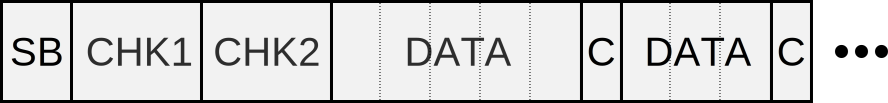
\includegraphics[width=0.45\textwidth, trim=0 3in 0 2in, clip]{./figures/lsvd.pdf}
    \caption{The LSVD file structure.}
    \label{fig:lsvd}
\end{figure}

\emph{Discussion on how versioning works, how we can retrieve arbitrary 
writes (change logs?) how we can easily extend this framework for snapshotting.}


\section{Evaluation}
\label{sec:evaluation}
\subsection{Methodology}
We ran our local experiments on a Dell Precision T7500n Dual Processor desktop 
computer running 64-bit RHEL6 built on the 2.6.32 kernel for CentOS6. The 
machine housed a Dual Quad Core Intel\textsuperscript{\textregistered} 
Xeon\textsuperscript{\textregistered} E5620 2.40GHz Processor, 24GB of RAM, 
two 600GB 15K RPM hard drives and one 2TB hard drive.

In remote case, we ran \XXX{Jim, care to fill this up?}

\subsection{LSVD microbenchmarks}
First, we wanted to evaluate our LSVD implementation. Since LSVD exports interface very similar to a file, we can easily compare LSVD throughput to regular file throughput. These benchmarks were all run locally.

We evaluated LSVD using five benchmarks, which we ran in specific order:
\begin{enumerate}
\item \textbf{Sequential write} - Sequential write of 5GB random data to a new file/LSVD with 40KB buffers,
\item \textbf{Sequential read} - Sequential read of 5GB of previously created file with 40KB buffers,
\item \textbf{Random read} - Randomly read 128MB using 4KB buffers,
\item \textbf{Random write} - Randomly written 128MB using 4KB buffers,
\item \textbf{Sequential read 2} - Sequential read of 5GB of the file using 40KB buffers. However, this time we are also reading changes made by fourth benchmark.
\end{enumerate}

All read and write operations were performed sequentially, without concurrency. Before read benchmarks, we cleared the file cache. Benchmarks were ran with LSVD checkpointing turned off.

Table \ref{tab:lsvd} shows benchmark results. As expected, we see very similar performances for sequential write, sequential read and random read benchmarks. Since LSVD turns all random writes into sequential writes, random writes executed on LSVD show throughput 52x larger than sequential writes on a normal file. However, LSVD pays the price of fast random writes on subsequent sequential reads of the data. Benchmark sequential read 2 read the whole file again, but now with 128MB of new writes at random places in the file. Benchmark on the file showed the same throughput as first time. However, random writes decreased LSVD sequential read throughput by 2.3x.


\begin{table}
\centering
\caption{LSVD microbenchmark results}
\label{tab:lsvd}
\begin{tabular}{ | l | r | r | }
\hline
\textbf{Benchmark} & \textbf{File (KB/s)} & \textbf{LSVD (KB/s)} \\
\hline
Sequential write & 121,297 & 120,143 \\
\hline
Sequential read & 194,323 & 194,407 \\
\hline
Random read & 1,202 & 1,189 \\
\hline
Random write & 2,097 & 109,493 \\
\hline
Sequential read 2 & 195,421 & 85,183 \\
\hline
\end{tabular}
\end{table}

\subsection{Checkpointing evaluation}
One of the important aspects of LSVD is checkpointing. We use it to keep recovery time from growing indefinitely. We designed an experiment to prove that our recovery time is bounded.

The experiment started with a write operation, which kept sending new updates to LSVD file until we killed it with \texttt{SIGKILL}. We then opened LSVD file and measured how long does a recovery take.

Figure \ref{fig:checkpointing} shows the results of the experiment. The horizontal axis shows runtime of the write before we killed it. Blue line shows time it took LSVD to recover to the state where it's able to receive new updates. Red line shows total data written during each experiment. When we ran the experiment for 150 seconds, it took LSVD 40 seconds to recover. However, when we ran the experiment for 200 seconds, recovery time was less than 5 seconds, even though we wrote more data to LSVD in total. These results show that our recovery time is bounded and does not grow linearly with number of updates or total data written. \XXX{say something about high recovery times at certain points}

\begin{figure}
  \centering
   \includegraphics[width=3.5in]{figures/checkpointing.pdf}
   \caption{Recovery time after writing data to LSVD file for a specific amount of time.}
   \label{fig:checkpointing}
\end{figure}

\subsection{File System Benchmarks}

\begin{figure}
  \centering
   \includegraphics[width=3.5in]{figures/benchmarks.pdf}
   \caption{File system benchmarks \XXX{TODO}}
   \label{fig:checkpointing}
\end{figure}


\section{Conclusion}
\label{sec:conc}
Presently, replicated block stores seem to be dominated by either DRBD-style or commercial NAS solutions. DRBD has the disadvantage that it is somewhat inflexible: it only allows two replicas (without stacking) and lacks dynamically resizing disk images. Further, DRBD puts all of its logic into a Linux kernel driver, making it more difficult to port to different systems. Commercial NAS solutions have the disadvantage of expense and opacity.

FreEBS shows that one can profitably move most of the replication logic into userspace programs. When the kernel driver becomes much simpler, it becomes more portable and reliable. Further, the replica managers themselves are more portable and maintainable. FreEBS is also a strong step in the direction of commoditizing replicated block storage for cloud computing since it enables such technology to be run on commodity hardware.

\bibliographystyle{plain}
\bibliography{biblio}

\end{document}



